\documentclass[a4paper,11pt]{article}
\usepackage[utf8]{inputenc}
\usepackage[french]{babel}
\usepackage[T1]{fontenc}
\usepackage{makeidx}
\makeindex
\usepackage{lmodern}
\usepackage{color}
\usepackage{graphicx}
\usepackage{listings}
\usepackage{caption}
\usepackage{subcaption}
 \usepackage{float}


\newcommand{\br}{\\\mbox{}}



\begin{document}

%\pagenumbering{gobble}

\title{\color{red}Projet Test et Vérification : \br\textbf{Test URI}}
\date{Décembre 2016}
\author{Sarra BOUTAHLIL\br Alexis DONNART}

\maketitle

\begin{abstract}
Dans le cadre du cours de Test et Vérification de Master 1 ALMA 2016-2017 dispensé à l'Université de Nantes par S. Gerson, il nous à été demandé d'évaluer et d'améliorer la qualité de la classe URI, qui fait partie du projet EMF (Eclipse Modeling Framework), dans le langage Java.
\end{abstract}
\pagebreak

\tableofcontents


\pagebreak 

\section{Analyse statique}
Première étape du test de la classe URI : l'analyse statique. On va s'attacher à analyser la syntaxe et les erreurs éventuelles que l'on pourrait trouver sans exécuter le code.
\subsection{Erreurs de syntaxe}
Nous utilisons dans un premier temps l'outil \textit{PMD} pour analyser la syntaxe et les bonnes pratiques du code.\br
De nombreuses corrections ont été apporté grâce à l'analyse de PMD.
\begin{itemize}
\item  \textbf{Parenthèses inutiles} mauvaise pratique la plus commune trouvé dans la classe URI, facilement corrigé en supprimant les parenthèses.
\item \textbf{Blocs vides} de nombreux blocs étaient vides : if, catch, \dots Nous avons simplement supprimé les blocs qui pouvaient l'être, et ajouté des logs d'erreur dans ceux qui ne pouvaient pas l'être.
\end{itemize}
En conclusion, des mauvaises pratiques facilement corrigés. Nous réutiliserons cet outil tout au lieu du test de la classe URI pour nous assurer de toujours respecter les bonnes pratiques de syntaxe.
\subsection{Bugs trouvés}
Nous avons ensuite utilisé \textit{FindBugs} pour tenter de détecter des bugs dans la syntaxe. Nous en avons détecté et corrigé plus de 40.
Parmis les plus courants : 
\begin{itemize}
\item Utilisation de l'opérateur \textit{==} plutôt que \textit{equals} ce qui pouvait conduire à des erreurs de comparaison.
\item Utilisation d'opérateurs \textit{synchronized} sans réels utilités.
\item Comparaison entre deux références du même objet : erreur de la part du développeur.
\end{itemize}
D'autres erreurs moins graves ont également été détecté grâce à cet outil, mais de nombreuses erreurs ont pu être corrigé avant même l'exécution.
\subsection{Évolutions à prévoir}
Dans l'analyse statique du code, nous avons pu approcher la classe URI et sa structure interne. Nous avons détecté de nombreux problèmes de conception.\br
La classe URI est une \textit{classe dieu}, elle contrôle tout et englobe toutes les autres classes et fonctionnalités. Il faudra découper cette classe et en extraire toutes les classes internes (6).\br
De même, certaines des classes internes de URI possèdent elles aussi de nombreuses classes internes. On extraira également ces classes.\br
De très nombreuses fonctionnalités de la classe URI ne sont pas implémentés et ne font que renvoyer \textit{true}, \textit{this} ou \textit{null}. Nous veillerons à tenir compte dans les tests de cette absence d'implémentation.
\section{Tests}
Dans un deuxième temps, nous allons tester la classe URI de façon dynamique puis nous évaluerons la qualité des tests.
\subsection{Tests unitaires}
Nous allons tenter de valider la classe URI à l'aide de test unitaires réalisés avec \textit{JUnit}.\br
La classe URI n'est qu'en partie testable du fait de la visibilité et de la contrôlabilité de ses états. Toutes les classes publiques et testables s'élèvent au compte de 43. Parmi toutes ces fonctions, nous dénombrons plusieurs cas de tests, pour un total de 100 tests.\br
Outre ces cas de tests, certaines fonctions sous tests ne correspondent pas à la spécification ou plantent (\textit{NullException}) quelque soit les cas testés, nous avons donc décidé de les annotés \textit{@Ignore}.\br
Nous avons également décidé d'annoter \textit{@Ignore} les fonctions accessible mais utilisant des fichiers, l'utilisation de fichier étant difficilement contrôlable et testable.
\subsection{Analyse des tests}
L'écriture des jeux de test finie, nous allons maintenant s'assurer de leur qualité en regardant la couverture et la mutation.
\subsubsection*{Couverture du code}
Pour assurer la couverture du code, nous utiliserons le plugin \textit{EclEmma} de Eclipse. Celui ci se charge de vérifier que toutes les branches du code sont couvertes par nos tests. Nous obtenons un score de couverture 71.5\% [\ref{Couv}].

\begin{figure}[h]
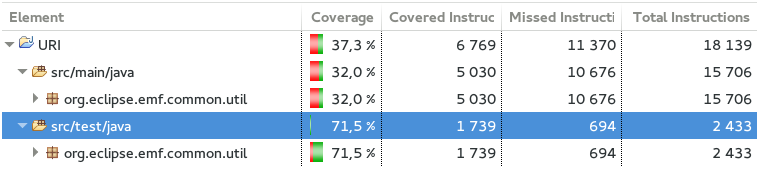
\includegraphics[scale=0.5]{Couverture.png}
\caption{Score de couverture de la suite de test de la classe URI}
\label{Couv}
\end{figure}

Ce score s'explique pour la majorité par l'absence de contrôlabilité sur tous les états du système. Notamment l'absence d'implémentation de nombreuses fonctions (qui renvoient toujours les même valeurs) ne nous permet pas de tester toutes les conditions, et ce quelque soit les valeurs d'entrées.

\subsubsection*{Analyse de mutation}

Dans un deuxième temps, nous allons muter le code pour s'assurer de la qualité de nos tests. Nous utilisons pour cela l'outil \textit{PIT} disponible sous Eclipse pour l'analyse de mutation.\br
Les tests de la classe URI obtiennent un score de 17\%, qui s'explique encore une fois par l'absence de contrôlabilité de l'état interne des fonctions, mais également par l'absence ou l'incohérence de la spécification des fonctions.

\section{Refactoring}

Avec les jeux de tests fonctionnels et leur qualité assuré, nous pouvons effectuer des modifications pour assurer une bonne conception. Nous utiliserons pour cela les outils de refactoring, dont ceux mis à disposition par Eclipse. Chaque refactoring impliquera une réexécution des tests unitaires ainsi que des outils de test statique (PMD, FindBugs).\br
Nous avons identifié précédemment les principaux problèmes de la classe URI à savoir qu'elle possède trop de comportement et trop de classes internes. Pour résoudre ce problème, nous créerons un nouveau type indépendant à partir de chaque classe interne. Ainsi les classes \textit{URIPool}, \textit{Opaque}, \textit{Fragment}, \textit{Hierarchical} et \textit{LazyFragmentInitializer} deviennent des classes à visibilité package indépendantes.\br
De ces classes, nous constatons encore la présence d'une \textit{classe dieu} : \textit{URIPool}. Nous allons donc en extraire toutes ses classes internes. Les classes \textit{AccessUnitBase}, \textit{StringAccessUnit}, \textit{PlateformAccessUnit}, \textit{FileAccessUnit}, \textit{ComponentAccessUnit} et \textit{CachedToString} deviennent également des classes indépendantes.\br
Nous constatons que dans toutes les classes implémentant \textit{AccessUnit}, une classe interne \textit{Queue}, presque similaire à toutes ces classes est présente. Nous allons donc extraire ces classes, les renommer spécifiquement du nom de la classe dont elle sont issues (\textit{ComponentQueue}, \dots) et en extraire les fonctions communes dans une super classe \textit{Queue}.\br
En dernier, nous voulions extraire toutes les données \textit{ final static} de la classe URI vers une classe de données, mais ce processus perdait la référence de certaines données, donc nous avons laisser les données tels quels.

\section{Conclusion}

La classe URI a été développé de façon approximative : non finie, des erreurs, du code qui ne respecte pas l'usage, \dots Grâce aux outils d'analyse statique et dynamique, nous avons pu valider le fonctionnement de certaines partie de cette classe, ou au contraire les invalider. Ces analyses ont finalement permis d'améliorer la conception de la classe à l'aide du Refactoring.

\end{document}
